\chapter{Text classification}


\section{Common tasks}

\begin{description}
    \item[Sentiment analysis/Opinion mining] \marginnote{Sentiment analysis/Opinion mining}
        Detection of attitudes. It can involve detecting:
        \begin{itemize}
            \item The holder of attitude (i.e., the source).
            \item The target of attitude (i.e., the aspect).
            \item The type of attitude (e.g., positive or negative).
            \item The text containing the attitude. 
        \end{itemize}

    \item[Spam detection]
    \item[Language identification]
    \item[Authorship attribution]
    \item[Subject category classification] 
\end{description}


\section{Classification}

\begin{description}
    \item[Classification task] \marginnote{Classification task}
        Given an input $x$ and a set of possible classes $Y = \{ y_1, \dots, y_M \}$, a classifier determines the class $\hat{y} \in Y$ associated to $x$.

        Classification can be:
        \begin{descriptionlist}
            \item[Rule-based] \marginnote{Rule-based}
                Based on fixed (possibly handwritten) rules.

                \begin{example}
                    Blacklist, whitelist, regex, \dots
                \end{example}

            \item[In-context learning] \marginnote{In-context learning}
                Provide a decoder (i.e., generative) large language model a prompt describing the task and the possible classes.

                \begin{example}
                    Zero-shot learning, few-shot learning, \dots
                \end{example}

            \item[Supervised machine learning] \marginnote{Supervised machine learning}
                Use a training set of $N$ labeled document-class data points $\{ (d_i, c_i) \}$ to fit a classifier.

                An ML model can be:
                \begin{descriptionlist}
                    \item[Generative] Informally, it learns the distribution of the data (i.e., $\prob{d_i | c_i}$).
                    \item[Discriminative] Informally, it learns to exploit the features to determine the class (i.e., $\prob{c_i | d_i}$).
                \end{descriptionlist}
        \end{descriptionlist}
\end{description}


\section{Naive Bayes}

\begin{description}
    \item[Bag-of-words (BoW)] \marginnote{Bag-of-words (BoW)}
        Representation of a document using the frequency of its words.

        Given a vocabulary $V$ and a document $d$, the bag-of-words embedding of $d$ is a vector in $\mathbb{N}^{\vert V \vert}$ where the $i$-th position contains the number of occurrences of the $i$-th token of $V$ in $d$.

    \item[Multinomial naive Bayes classifier] \marginnote{Multinomial naive Bayes classifier}
        Generative probabilistic classifier based on the assumption that features are independent given the class.

        Given a document $d = \{ w_1, \dots, w_n \}$, a naive Bayes classifier returns the class $\hat{c}$ with maximum posterior probability:
        \[
            \begin{split}
                \hat{c} &= \arg\max_{c \in C} \prob{c | d} \\
                &= \arg\max_{c \in C} \underbrace{\prob{d | c}}_{\text{likelihood}} \underbrace{\prob{c}}_{\text{prior}} \\
                &= \arg\max_{c \in C} \prob{w_1, \dots, w_n | c} \prob{c} \\
                &\approx \arg\max_{c \in C} \prod_{i} \prob{w_i | c} \prob{c} \\
                &= \arg\max_{c \in C} \sum_{i} \log\prob{w_i | c} \log\prob{c} \\
            \end{split}
        \]

        Given a training set $D$ and a vocabulary $V$, $\prob{w_i | c}$ and $\prob{c}$ are determined during training by maximum likelihood estimation as follows:
        \[
            \prob{c} = \frac{N_c}{\vert D \vert}
            \qquad
            \prob{w_i | c} = \frac{\texttt{count}(w_i, c)}{\sum_{v \in V} \texttt{count}(v, c)}
        \]
        where $N_c$ is the number of documents of class $c$ and $\texttt{count}(w, c)$ counts the occurrences of the word $w$ in the training samples of class $c$.

        \begin{remark}
            Laplace smoothing is used to avoid zero probabilities.
        \end{remark}

        \begin{remark}
            Stop words can be removed from the training set as they are usually not relevant.
        \end{remark}

        \begin{remark}
            The likelihood part of the equation ($\sum_{i} \log\prob{w_i | c}$) can be seen as a set of class-specific 1-gram language models.
        \end{remark}
\end{description}

\begin{example}
    Given the following training set for sentiment analysis with two classes:
    \begin{table}[H]
        \centering
        \footnotesize
        \begin{tabular}{cl}
            \toprule
            \textbf{Class} & \textbf{Document} \\
            \midrule
            \texttt{-} & \texttt{just plain boring} \\
            \texttt{-} & \texttt{entirely predictable and lacks energy} \\
            \texttt{-} & \texttt{no surprises and very few laughs} \\
            \texttt{+} & \texttt{very powerful} \\
            \texttt{+} & \texttt{the most fun film of the summer} \\
            \bottomrule
        \end{tabular}
    \end{table}
    We want to classify the sentence ``\texttt{predictable with no fun}''. Excluding stop words (i.e., \texttt{with}), we need to compute:
    \[
        \begin{split}
            \prob{\texttt{+} | \texttt{predictable with no fun}} &= \prob{\texttt{+}} \prob{\texttt{predictable} | \texttt{+}} \prob{\texttt{no} | \texttt{+}} \prob{\texttt{fun} | \texttt{+}} \\
            \prob{\texttt{-} | \texttt{predictable with no fun}} &= \prob{\texttt{-}} \prob{\texttt{predictable} | \texttt{-}} \prob{\texttt{no} | \texttt{-}} \prob{\texttt{fun} | \texttt{-}}
        \end{split}
    \]
    A vocabulary of $20$ tokens can be used to represent the training samples. The required likelihoods and priors with Laplace smoothing are computed as:
    \[
        \begin{gathered}
            \prob{\texttt{+}} = \frac{2}{5} \qquad \prob{\texttt{predictable} | \texttt{+}} = \frac{0+1}{9+20} \quad \prob{\texttt{no} | \texttt{+}} = \frac{0+1}{9+20} \quad \prob{\texttt{fun} | \texttt{+}} = \frac{1+1}{9+20} \\
            \prob{\texttt{-}} = \frac{3}{5} \qquad \prob{\texttt{predictable} | \texttt{-}} = \frac{1+1}{14+20} \quad \prob{\texttt{no} | \texttt{-}} = \frac{1+1}{14+20} \quad \prob{\texttt{fun} | \texttt{-}} = \frac{0+1}{14+20}
        \end{gathered}
    \]
\end{example}


\subsection{Optimizations}

Possible optimizations for naive Bayes applied to sentiment analysis are the following:
\begin{descriptionlist}
    \item[Binarization] \marginnote{Binarization}
        Generally, the information regarding the occurrence of a word is more important than its frequency. Therefore, instead of applying bag-of-words by counting, it is possible to produce a one-hot encoded vector to indicate which words are in the document.

    \item[Negation encoding] \marginnote{Negation encoding}
        To encode negations, two approaches can be taken:
        \begin{description}
            \item[Negation annotation]
                Add to negated words an annotation so that they are treated as a new word.
                \begin{example}
                    Prepend \texttt{NOT\char`_} to each word between a negation and the next punctuation:
                    \[ \text{didn't like this movie.} \mapsto \text{didn't \texttt{NOT\char`_}like \texttt{NOT\char`_}this \texttt{NOT\char`_}movie.} \]
                \end{example}

            \item[Parse tree]
                Build a tree to encode the sentiment and interactions of the words. By propagating the sentiments bottom-up, it is possible to determine the overall sentiment of the sequence.

                \begin{example}
                    The parse tree for the sentence ``\texttt{This film doesn't care about cleverness, wit or any other kind of intelligent humor.}'' is the following:
                    \begin{figure}[H]
                        \centering
                        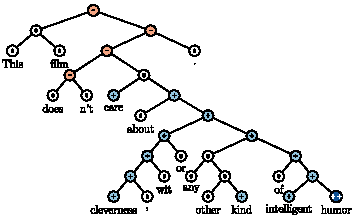
\includegraphics[width=0.6\linewidth]{./img/_sentiment_parse_tree.pdf}
                    \end{figure}
                    Due to the negation (\texttt{doesn't}), the whole positive sequence is negated.
                \end{example}
        \end{description}

    \item[Sentiment lexicon] \marginnote{Sentiment lexicon}
        If training data is insufficient, external domain knowledge, such as sentiment lexicon, can be used.

        \begin{example}
            A possible way to use a lexicon is to count the number of positive and negative words according to that corpus.
        \end{example}

        \begin{remark}
            Possible ways to create a lexicon are through:
            \begin{itemize}
                \item Expert annotators.
                \item Crowdsourcing in a two-step procedure:
                    \begin{enumerate}
                        \item Ask questions related to synonyms (e.g., which word is closest in meaning to \textit{startle}?).
                        \item Rate the association of words with emotions (e.g., how does \textit{startle} associate with \textit{joy}, \textit{fear}, \textit{anger}, \dots?).
                    \end{enumerate}
                \item Semi-supervised induction of labels from a small set of annotated data (i.e., seed labels). It works by looking for words that appear together with the ones with a known sentiment.
                \item Supervised learning using annotated data.
            \end{itemize}
        \end{remark}
\end{descriptionlist}


\subsection{Properties}

Naive Bayes has the following properties:
\begin{itemize}
    \item It is generally effective with short sequences and fewer data samples.
    \item It is robust to irrelevant features (i.e., words that appear in both negative and positive sentences) as they cancel out each other.
    \item It has good performance in domains with many equally important features (contrarily to decision trees).
    \item The independence assumption might produce overestimated predictions.
\end{itemize}

\begin{remark}
    Naive Bayes is a good baseline when experimenting with text classifications.
\end{remark}



\section{Logistic regression}

\begin{description}
    \item[Features engineering] \marginnote{Features engineering}
        Determine features by hand from the data (e.g., number of positive and negative lexicon).


    \item[Binary logistic regression] \marginnote{Binary logistic regression}
        Discriminative probabilistic model that computes the joint distribution $\prob{c | d}$ of the class $c$ given the document $d$.

        Given the input features $\vec{x} = [x_1, \dots, x_n]$, logistic regression computes the following:
        \[ 
            \sigma\left( \sum_{i=1}^{n} w_i x_i + b \right) = \sigma(\vec{w}\vec{x} + b)
        \]
        where $\sigma$ is the sigmoid function.

        \begin{description}
            \item[Loss]
                The loss function should aim to maximize the probability of predicting the correct label $\hat{y}$ given the observation $\vec{x}$. This can be expressed as a Bernoulli distribution:
                \[ 
                    \prob{y | x} = \hat{y}^y (1-\hat{y})^{1-y} = \begin{cases}
                        1 - \hat{y} & \text{if $y=0$} \\
                        \hat{y} & \text{if $y=1$} \\
                    \end{cases} 
                \]
                By applying a log-transformation and inverting the sign, this corresponds to the cross-entropy loss in the binary case:
                \[ \mathcal{L}_{\text{BCE}}(\hat{y}, y) = -\log(\prob{y | x}) = -[y \log(\hat{y}) + (1-y)\log(1-\hat{y})] \]

            \item[Optimization]
                As cross-entropy is convex, SGD is well suited to find the parameters $\vec{\theta}$ of a logistic regressor $f$ over batches of $m$ examples by solving:
                \[ \arg\min_{\vec{\theta}} \sum_{i=1}^{m} \mathcal{L}_\text{BCE}(\hat{y}^{(i)}, f(x^{(i)}; \vec{\theta})) + \alpha \mathcal{R}(\vec{\theta}) \]
                where $\alpha$ is the regularization factor and $\mathcal{R}(\vec{\theta})$ is the regularization term. Typical regularization approaches are:
                \begin{descriptionlist}
                    \item[Lasso regression (L1)] $\mathcal{R}(\vec{\theta}) = \Vert \vec{\theta} \Vert_1 = \sum_{j=1}^{n} \vert \vec{\theta}_j \vert$.
                    \item[Ridge regression (L2)] $\mathcal{R}(\vec{\theta}) = \Vert \vec{\theta} \Vert^2_2 = \sum_{j=1}^{n} \vec{\theta}_j^2$.
                \end{descriptionlist}
        \end{description}

    \item[Multinomial logistic regression] \marginnote{Multinomial logistic regression}
        Extension of logistic regression to the multi-class case. The joint probability becomes $\prob{y = c | x}$ and softmax is used in place of the sigmoid.

        Cross-entropy is extended over the classes $C$:
        \[ \mathcal{L}_\text{CE}(\hat{y}, y) = - \sum_{c \in C} \mathbbm{1}\{y = c\} \log(\prob{y = c | x}) \]
\end{description}


\subsection{Properties}

Logistic regression has the following properties:
\begin{itemize}
    \item It is generally effective with large documents or datasets.
    \item It is robust to correlated features.
\end{itemize}

\begin{remark}
    Logistic regression is also a good baseline when experimenting with text classification. 
    
    As they are lightweight to train, it is a good idea to test both naive Bayes and logistic regression to determine the best baseline for other experiments.
\end{remark}



\section{Metrics}


\subsection{Binary classification}

\begin{description}
    \item[Contingency table] \marginnote{Contingency table}
        $2 \times 2$ table matching predictions to ground truths. It contains true positives (\texttt{TP}), false positives (\texttt{FP}), false negatives (\texttt{FN}), and true negatives (\texttt{TN}).

    \item[Recall] \marginnote{Recall} 
        $\frac{\texttt{TP}}{\texttt{TP} + \texttt{FN}}$.

    \item[Precision] \marginnote{Precision} 
        $\frac{\texttt{TP}}{\texttt{TP} + \texttt{FP}}$.

    \item[Accuracy] \marginnote{Accuracy} 
        $\frac{\texttt{TP} + \texttt{TN}}{\texttt{TP} + \texttt{FP} + \texttt{FN} + \texttt{TN}}$.

        \begin{remark}
            Accuracy is a reasonable metric only when classes are balanced.
        \end{remark}

    \item[F1 score] \marginnote{F1 score} 
        $\frac{2 \cdot \texttt{recall} \cdot \texttt{precision}}{\texttt{recall} + \texttt{precision}}$.
\end{description}


\subsection{Multi-class classification}

\begin{description}
    \item[Confusion matrix] \marginnote{Confusion matrix}
        $c \times c$ table matching predictions to ground truths.

    \item[Precision/Recall] \marginnote{Precision/Recall}
        Precision and recall can be defined class-wise (i.e., consider a class as the positive label and the others as the negative).

    \item[Micro-average precision/recall] \marginnote{Micro-average precision/recall}
        Compute the contingency table of each class and collapse them into a single table. Compute precision or recall on the pooled contingency table.

        \begin{remark}
            This approach is sensitive to the most frequent class.
        \end{remark}

    \item[Macro-average precision/recall] \marginnote{Macro-average precision/recall}
        Compute precision or recall class-wise and then average over the classes.

        \begin{remark}
            This approach is reasonable if the classes are equally important.
        \end{remark}

        \begin{remark}
            Macro-average is more common in NLP.
        \end{remark}
\end{description}

\begin{example}
    \phantom{}

    \begin{figure}[H]
        \centering
        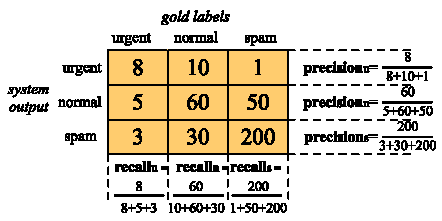
\includegraphics[width=0.5\linewidth]{./img/_confusion_matrix_example.pdf}
        \caption{Confusion matrix}
    \end{figure}

    \begin{figure}[H]
        \centering
        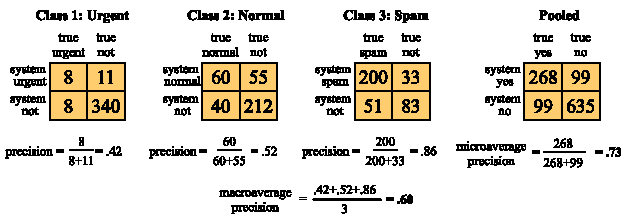
\includegraphics[width=0.85\linewidth]{./img/_micro_macro_average_example.pdf}
        \caption{
            \parbox[t]{0.6\linewidth}{
                Class-wise contingency tables, pooled contingency table, and micro/macro-average precision
            }
        }
    \end{figure}
\end{example}


\subsection{Cross-validation}

\begin{description}
    \item[$\mathbf{n}$-fold cross-validation] \marginnote{$n$-fold cross-validation}
        Tune a classifier on different sections of the training data:
        \begin{enumerate}
            \item Randomly choose a training and validation set.
            \item Train the classifier.
            \item Evaluate the classifier on a held-out test set.
            \item Repeat for $n$ times.
        \end{enumerate}
\end{description}

\subsection{Statistical significance}

\begin{description}
    \item[$\mathbf{p}$-value] \marginnote{$p$-value}
        Measure to determine whether a model $A$ is outperforming a model $B$ on a given test set by chance (i.e., test the null hypothesis $H_0$ or, in other words, test that there is no relation between $A$ and $B$).

        Given:
        \begin{itemize}
            \item A test set $x$,
            \item A random variable $X$ over the test sets (i.e., another test set),
            \item Two models $A$ and $B$, such that $A$ is better than $B$ by $\delta(x)$ on the test set $x$,
        \end{itemize}
        the $p$-value is defined as:
        \[ p\text{-value}(x) = \prob{\delta(X) > \delta(x) | H_0} \]
        There are two cases:
        \begin{itemize}
            \item $p\text{-value}(x)$ is big: the null hypothesis holds (i.e., $\prob{\delta(X) > \delta(x)}$ is high under the assumption that $A$ and $B$ are not related), so $A$ outperforms $B$ by chance.
            \item $p\text{-value}(x)$ is small (i.e., $< 0.05$ or $< 0.01$): the null hypothesis is rejected, so $A$ actually outperforms $B$.
        \end{itemize}

    \item[Bootstrapping test] \marginnote{Bootstrapping test}
        Approach to compute $p$-values.

        Given a test set $x$, multiple virtual test sets $\bar{x}^{(i)}$ are created by sampling with replacement (it is assumed that the new sets are representative). The performance difference $\delta(\cdot)$ is computed between two models and the $p$-value is determined as the frequency of:
        \[ \delta(\bar{x}^{(i)}) > 2\delta(x) \]

        \begin{remark}
            $\delta(x)$ is doubled due to theoretical reasons.
        \end{remark}

        \begin{example}
            Consider two models $A$ and $B$, and a test set $x$ with 10 samples. From $x$, multiple new sets (in this case of the same size) can be sampled. In the following table, each cell indicates which model correctly predicted the class:
            \begin{center}
                \footnotesize
                \begin{tabular}{ccccccccccc|ccc}
                    \toprule
                                    & 1 & 2 & 3 & 4 & 5 & 6 & 7 & 8 & 9 & 10 & $A\%$ & $B\%$ & $\delta(\cdot)$ \\
                    \midrule
                    $x$             & $AB$ & $A$ & $AB$ & $B$ & $A$ & $B$ & $A$ & $AB$ & -- & $A$ & $0.7$ & $0.5$ & $0.2$ \\
                    $\bar{x}^{(1)}$   & $A$ & $AB$ & $A$ & $B$ & $B$ & $A$ & $B$ & $AB$ & -- & $AB$ & $0.6$ & $0.6$ & $0.0$ \\
                    $\vdots$ & $\vdots$ & $\vdots$ & $\vdots$ & $\vdots$ & $\vdots$ & $\vdots$ & $\vdots$ & $\vdots$ & $\vdots$ & $\vdots$ & $\vdots$ & $\vdots$ & $\vdots$ \\
                    \bottomrule
                \end{tabular}
            \end{center}
            A possible way to sample $\bar{x}^{(1)}$ is (w.r.t. the indexes of the examples in $x$) $[2, 3, 3, 2, 4, 6, 2, 4, 1, 9, 1]$.
        \end{example}
\end{description}



\section{Affective meaning} \label{sec:affective_meaning}

The affective meaning of a text corpus can vary depending on:
\begin{descriptionlist}
    \item[Personality traits] 
        Stable behavior and personality of a person (e.g., nervous, anxious, reckless, \dots).

    \item[Attitude] 
        Enduring sentiment towards objects or people (e.g., liking, loving, hating, \dots).

    \item[Interpersonal stance] 
        Affective stance taken in a specific interaction (e.g., distant, cold, warm, \dots).

    \item[Mood] 
        Affective state of low intensity and long duration often without an apparent cause (e.g., cheerful, gloomy, irritable, \dots).

    \item[Emotion] 
        Brief response to an external or internal event of major significance (e.g., angry, sad, joyful, \dots).

        \begin{remark}
            Emotion is the most common subject in affective computing.
        \end{remark}
\end{descriptionlist}


\subsection{Emotion}

\begin{description}
    \item[Theory of emotion]
        There are two main theories of emotion:
        \begin{descriptionlist}
            \item[Basic emotions] \marginnote{Basic emotions}
                Discrete and fixed range of atomic emotions.

                \begin{remark}
                    Emotions associated to a word might be in contrast. For instance, in the NRC Word-Emotion Association Lexicon the word \texttt{thirst} is associated to both \textit{anticipation} and \textit{surprise}.
                \end{remark}

            \item[Continuum emotions] \marginnote{Continuum emotions}
                Describe emotions in a 2 or 3 dimensional space with the following features:
                \begin{descriptionlist}
                    \item[Valence] Pleasantness of a stimulus.
                    \item[Arousal] Intensity of emotion.
                    \item[Dominance] Degree of control on the stimulus.
                \end{descriptionlist}

                \begin{remark}
                    Valence is often used as a measure of sentiment.
                \end{remark}
        \end{descriptionlist}
\end{description}